\begin{pr}$ $
\newcommand{\w}{{\overline\omega}}
\begin{enumerate}[(a)]
\item Consider $\phi_{\tau, \gamma}(x):=\begin{cases}
1\text{, if }LR(x)>\tau\\
\gamma\text{, if }LR(x)=\tau\\
0\text{, if }LR(x)<\tau
\end{cases}$.\\
$LR(0)=\frac{P_1(0)}{P_0(0)}=\frac{1-p_1}{1-p_0}$.\\
$LR(1)=\frac{P_1(1)}{P_0(1)}=\frac{p_1}{p_0}$.\\
$\cuz p_0<p_1$.\\
$\so LR(1)=\frac{p_1}{p_0}>1>\frac{1-p_1}{1-p_0}=LR(0)$.\\
By Neyman-Pearson theorem, $\phi_{\tau, \gamma}$ is optimal.\\
$\pi_{1|0}(\phi_{\tau, \gamma})=P_0\{LR(X)>\tau\}+\gamma P_0\{LR(X)=\tau\}$.\\
$\pi_{0|1}(\phi_{\tau, \gamma})=P_1\{LR(X)<\tau\}+(1-\gamma)P_1\{LR(X)=\tau\}$.\\
We only need to consider the cases $\tau=LR(x)$ for some $x$, since other cases can be reduced to these cases by setting $\gamma$ properly.\\
For $\tau=LR(0)$, $\pi_{1|0}=P_0(1)+\gamma P_0(0)=p_0+\gamma(1-p_0)$; $\pi_{0|1}=0+(1-\gamma)P_1(0)=(1-\gamma)(1-p_1)$.\\
For $\tau=LR(1)$, $\pi_{1|0}=0+\gamma P_0(1)=\gamma p_0$; $\pi_{0|1}=P_1(0)+(1-\gamma)P_1(1)=1-p_1+(1-\gamma)p_1$.\\
The above forms two segments, and their intersection is $(p_0, 1-p_1)$, which can be calculated by setting $\gamma$ in the first segment to $0$ or in the second segment to $1$.\\
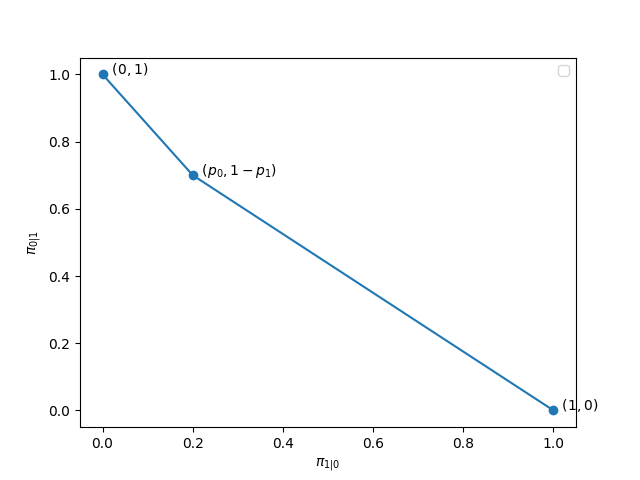
\includegraphics[width=15cm]{1a.png}
\item Let $Y$ be the random variable denoting the length of the observed sequence. We can see that $P_Y(y)=p(1-p)^{y-1}$.\\
$P\{Y>y\}=\suml_{z=y+1}^\infty p(1-p)^{z-1}=\frac{p(1-p)^y}{1-(1-p)}=(1-p)^y$.\\
$P\{Y<y\}=\suml_{z=1}^{y-1}p(1-p)^{z-1}=\frac{p(1-(1-p)^{y-1})}{1-(1-p)}=1-(1-p)^{y-1}$.\\
$P_0(y)=p_0(1-p_0)^{y-1}, P_1(y)=p_1(1-p_1)^{y-1}$.\\
Consider $\phi_{\tau, \gamma}(y):=\begin{cases}
1\text{, if }LR(y)>\tau\\
\gamma\text{, if }LR(y)=\tau\\
0\text{, if }LR(y)<\tau
\end{cases}$.\\
$LR(y)=\frac{P_1(y)}{P_0(y)}=\frac{p_1(1-p_1)^{y-1}}{p_0(1-p_0)^{y-1}}$.\\
Since $p_0<p_1$, there is $\frac{1-p_1}{1-p_0}<1$.\\
$\then LR(y)$ is an decreasing function of $y$.\\
By Neyman-Pearson theorem, $\phi_{\tau, \gamma}$ is optimal.\\
We only need to consider the cases $\tau=LR(y)$ for some $y$, since other cases can be reduced to these cases by setting $\gamma$ properly.\\
Since $LR(y)$ is decreasing, for $\tau=LR(y),\ \pi_{1|0}(\phi_{\tau, \gamma})=P_0\{Y<y\}+\gamma P_0\{Y=y\}=1-(1-p_0)^{y-1}+\gamma p_0(1-p_0)^{y-1}=1-(1-p_0)^{y-1}(1-\gamma p_0)$.\\
$\pi_{0|1}(\phi_{\tau, \gamma})=P_1\{Y>y\}+(1-\gamma)P_1\{Y=y\}=(1-p_1)^y+(1-\gamma)p_1(1-p_1)^{y-1}=(1-\gamma p_1)(1-p_1)^{y-1}$.\\
For each $y$, it forms a segment, where the intersection of the segments formed by $y$ and $y+1$ is $(1-(1-p_0)^y, (1-p_1)^y)$, which can be calculated by setting $\gamma$ in the segment formed by $y$ to $1$ or in the other segment to $0$.\\
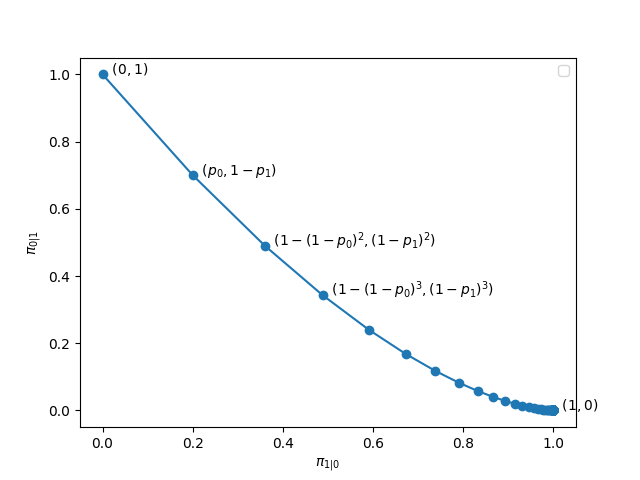
\includegraphics[width=15cm]{1b.png}
\item Let $Y_i$ be the random variable denoting the length of the sequence between the $i-1$-th $1$ and the $i$-th $1$ (including the $i$-th $1$ and excluding the $i-1$-th $1$).\\
One can see that $Y_i$ are i.i.d. and $Y_i\sim G(p)$.\\
Clearly, $Z=Y_1+Y_2+\cdots+Y_n$ is the random variable of the length of the observed sequence.\\
Let $Q_0=G(p_0), Q_1=G(p_1)$.\\
From Chernoff-Stein lemma, $\lim_{n\to\infty}-\frac1n\log\w_{0|1}^*(n, \epsilon)=\E_{Y\sim G(p_0)}[\log\frac{Q_0(Y)}{Q_1(Y)}]=\suml_{i=1}^\infty p_0(1-p_0)^{i-1}\log\frac{p_0(1-p_0)^{i-1}}{p_1(1-p_1)^{i-1}}=\suml_{i=1}^\infty p_0(1-p_0)^{i-1}\log\frac{p_0}{p_1}+\suml_{i=1}^\infty(i-1)p_0(1-p_0)^{i-1}\log\frac{1-p_0}{1-p_1}=p_0\frac1{1-(1-p_0)}\log\frac{p_0}{p_1}+p_0\log\frac{1-p_0}{1-p_1}\suml_{i=1}^\infty\suml_{j=1}^{i-1}(1-p_0)^{i-1}=\log\frac{p_0}{p_1}+p_0\log\frac{1-p_0}{1-p_1}\suml_{j=1}^\infty\suml_{i=j+1}^\infty(1-p_0)^{i-1}=\log\frac{p_0}{p_1}+p_0\log\frac{1-p_0}{1-p_1}\suml_{j=1}^\infty\frac{(1-p_0)^j}{p_0}=\log\frac{p_0}{p_1}+p_0\log\left(\frac{1-p_0}{1-p_1}\right)\frac{1-p_0}{p_0^2}=\log\frac{p_0}{p_1}+(\frac1{p_0}-1)\log\frac{1-p_0}{1-p_1}$.
%Let $Y$ be the random variable denoting the length of the observed sequence. The probability that a given sequence with length $y$ and $n$ $1$s appears is $p^n(1-p)^{y-n}$, and there are $\binom yn$ sequences of this kind.\\
%$\so P\{Y=y\}=\binom ynp^n(1-p)^{y-n}$.\\
%Note that if $a<b$ or $b<0$, then $\binom ab$ is defined as $0$.\\
%Let $f(n, y):=P\{Y<y\}=\suml_{z=0}^{y-1}\binom znp^n(1-p)^{z-n}$.\\
%Note that if $a<b$ or $b<0$, then $\binom ab$ is defined as $0$.\\
%$f(n, y)-(1-p)f(n, y-1)=p^n\suml_{z=0}^{y-1}(\binom zn-\binom{z-1}n)(1-p)^{z-n}=p^n\suml_{z=0}^{y-1}\binom{z-1}{n-1}(1-p)^{z-n}=p(1-p)f(n-1, y-1)$.\\
%Claim: $f(n, y)=p^{n-1}$
%In (b), we know that $f(1, y)=1-(1-p)^{y-1}$.\\
%Consider $\phi_{\tau, \gamma}(y):=\begin{cases}
%1\text{, if }LR(y)>\tau\\
%\gamma\text{, if }LR(y)=\tau\\
%0\text{, if }LR(y)<\tau
%\end{cases}$.\\
%$LR(y)=\frac{P_1(y)}{P_0(y)}=\frac{\binom ynp_1^n(1-p_1)^{y-n}}{\binom ynp_0^n(1-p_0)^{y-n}}=\frac{p_1^n(1-p_1)^{y-n}}{p_0^n(1-p_0)^{y-n}}$.\\
%Since $p_0<p_1$, there is $\frac{1-p_1}{1-p_0}<1$.\\
%$\then LR(y)$ is an decreasing function of $y$.\\
%By Neyman-Pearson theorem, $\phi_{\tau, \gamma}$ is optimal.\\
%We only need to consider the cases $\tau=LR(y)$ for some $y$, since other cases can be reduced to these cases by setting $\gamma$ properly.\\
%Since $LR(y)$ is decreasing, for $\tau=LR(y),\ \pi_{1|0}(\phi_{\tau, \gamma})=P_0\{Y<y\}+\gamma P_0\{Y=y\}=\suml_{z=0}^{y-1}\binom znp_0^n(1-p_0)^{z-n}+\gamma\binom ynp_0^n(1-p_0)^{y-n}$.\\
%$\pi_{0|1}(\phi_{\tau, \gamma})=P_1\{Y>y\}+(1-\gamma)P_1\{Y=y\}=\suml_{z=y+1}^\infty\binom znp_1^n(1-p_1)^{z-n}+(1-\gamma)\binom ynp_1^n(1-p_1)^{y-n}$.\\
%The optimal solution is $\pi_{1|0}(\phi_{\tau, \gamma})=\suml_{z=0}^{y-1}\binom znp_0^n(1-p_0)^{z-n}+\gamma\binom ynp_0^n(1-p_0)^{y-n}=\epsilon$, where $y$ is the minimum integer such that $\suml_{z=0}^y\binom znp_0^n(1-p_0)^{z-n}\geq\epsilon$.\\
%$\then\suml_{z=0}^y\binom znp_1(1-p_1)^{z-n}$
%$\pi_{0|1}(\phi_{\tau, \gamma})$
\end{enumerate}
\end{pr}
